\section{Data}
\label{sec:data}

EHRSHOT is a de-identified EHR dataset released by Stanford together with a set of clinical prediction tasks~\cite{wornow2023ehrshot}. We use the course's trimmed version, stored in the OMOP format, a shared layout for organising visits, diagnoses, and other medical records~\cite{hripcsak2015ohdsi}. It covers 6,731 patients, 944,132 visits, and 2.57 million diagnosis records.

\subsection{Two prediction questions}

We study two EHRSHOT tasks. The \emph{prediction time} is the moment the question is asked, and the \emph{label} is the true answer.
\begin{itemize}
  \item \textbf{Long stay.} At the end of the admission day, will this hospital stay last 7 days or more?
  \item \textbf{New high blood pressure.} At discharge, will the patient be diagnosed with essential hypertension for the first time within a year? Patients who already have the diagnosis are skipped.
\end{itemize}
The trimmed data do not include ready-made labels, so we rebuilt them from the EHRSHOT definitions. Where our labels and Stanford's official labels cover the same stays, they agree 99.84\% (long stay) and 99.40\% (high blood pressure) of the time (Table~\ref{tab:labels}).

\begin{table}[!htbp]
\centering
\caption{The two prediction questions.}
\label{tab:labels}
\small
\begin{tabular}{lrrr}
\toprule
Question & Stays & Patients & Positive \\
\midrule
Long stay ($\geq$ 7 days) & 6,998 & 3,844 & 25.4\% \\
New high blood pressure   & 3,511 & 2,217 & 12.8\% \\
\bottomrule
\end{tabular}
\end{table}

Each node in our patient networks is one hospital stay at its prediction time. A patient with several stays appears as several nodes, which matters later because two stays of the same person tend to look alike.

\subsection{Two kinds of diagnosis codes}

Diagnoses are recorded as billing codes. In October 2015, US hospitals switched from the older ICD-9 codes to the newer ICD-10 codes (Figure~\ref{fig:codes}), so the same disease can have a different code depending on the year. The OMOP format also maps both versions to a single \emph{standardised diagnosis code} from the SNOMED vocabulary. We use standardised codes for all main analyses, so that a diagnosis made in 2014 and the same diagnosis made in 2017 count as the same thing. Section~\ref{sec:robust} shows what goes wrong otherwise.

\begin{figure}[!htbp]
\centering
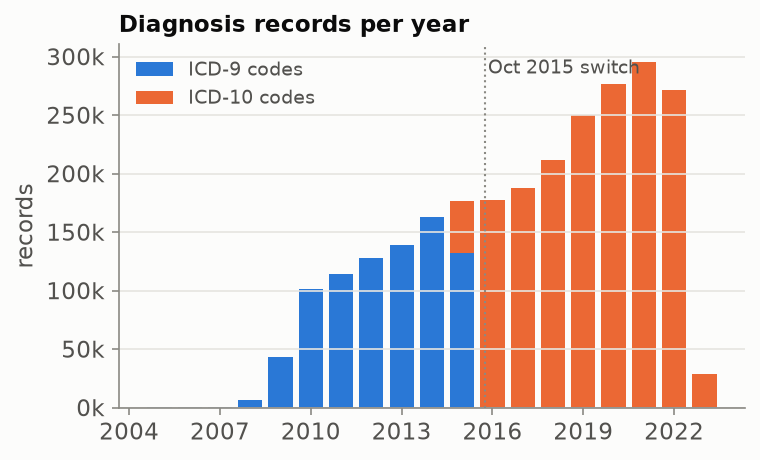
\includegraphics[width=\columnwidth]{01_billing_codes_by_year.png}
\caption{Diagnosis records per year. Hospitals switched from ICD-9 (blue) to ICD-10 (orange) billing codes in October 2015.}
\label{fig:codes}
\end{figure}
